\subsection{Asignatura curso académico}

  \paragraph{}Se procede a crear las asignaturas curso académico para las
  asignaturas en las que se matricula el alumno,
  en este caso, las mencionadas en el capítulo \ref{enunciado},
  \textit{Enunciado}, durante el curso académico 2010. Para ello, se realizará
  la creación de las asignaturas curso académico, tal y como se describió en el
  capítulo \ref{addAsignaturaCA}, \textit{Añadir asignatura curso académico}.

  \paragraph{}Una vez que aparezca el formulario de creación, se debe introducir
  el curso académico para cada asignatura, con lo que la pantalla quedaría tal
  y como refleja la figura \ref{ejemploAddAsignaturaCA} para el caso de la
  asignatura \textit{Biología molecular}. El resto de asignaturas siguen el
  mismo proceso de creación, con sus respectivos detalles.

  \begin{figure}[!ht]
    \begin{center}
      \fbox{
      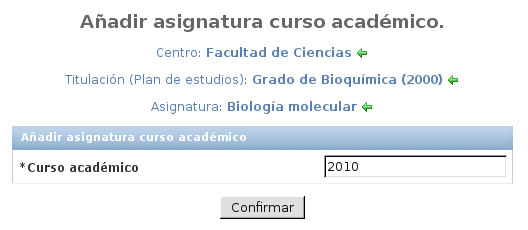
\includegraphics[scale=0.55]{5.Ejemplos_Practicos/5.3.IntroduccionDatos/5.3.4.AsignaturaCA/add_asignaturaCA.png}
      }
      \caption{Creación de \textit{Asignatura curso académico} de ejemplo.}
      \label{ejemploAddAsignaturaCA}
    \end{center}
  \end{figure}

  \paragraph{}Una vez rellenado el formulario, se pulsará el botón
  \textit{Confirmar}, el cual se puede ver en la figura
  \ref{capturaBotonConfirmar}. Si el formulario rellenado es válido, y no tiene
  errores, se creará el nuevo elemento en el sistema. En caso de contener
  información no válida, un mensaje de error aparecerá indicando los campos
  del formulario que no han pasado la validación, los cuales habrá que modificar
  para introducir correctamente el elemento en el sistema.
